\documentclass[12pt]{article}

\usepackage[utf8]{inputenc}
\usepackage[T1]{fontenc}
\usepackage{geometry}
\usepackage{graphicx} %figures
\usepackage{subfig} %subfigures
\usepackage{gensymb} %degree sign
\usepackage{amsmath} %math stuff
\usepackage{bm} %bold stuff
\geometry{a4paper}

\title{\textbf{Part 3: Radial Basis Functions}}

\begin{document}
\date{December 28, 2020}
\maketitle

I would like to quickly thank everyone for reading my last post about Gaussian processes and Bayesian optimization. It was a lot of fun to do and I hope everyone likes the code I provided. This week we are going over radial basis functions (RBFs). An RBF is a model structure that, much like Gaussian processes, relates some input of interest $x$ to some output of interest $y$ by relating a value of interest $x$ to training data $X$ and $Y$. In this case, that "relationship" is radial, in that it is distance based, such as with the much-beloved L2 norm $r=||x-X||_2^2$. Point that are closer have smaller $r$ values, so are going to be modeled as more similar to one another. This is quite similar to Gaussian processes, so hopefully the qualitative concept is fresh in everyone's mind.

\section{Radial Basis Function Model}

The basic model of an RBF is as follows:

\begin{equation}
\hat{y}=\Sigma_{i=1}^{n_c} \lambda_i \phi(r_i)
\end{equation}

\begin{align*}
r=||\hat{x}-x_c||_2^2
\end{align*}

Notice we have added $\phi$, which is the activation function that takes some $r$ and projects it into output space. Common activation functions are exponential/Gaussian $\phi(r)=exp(-\sigma^2 r)$, or the cubic $\phi(r)=r^3$, or the thin plate spline $\phi(r)=r^2 ln(r)$. In Figures 1 and 2 we can see that as one moves away from the "center" located at $x=0.5$, or as $r$ increases, $\phi$ changes as well. 

\vspace{5mm}

As a note, it doesn't matter if $\phi$ increases or decreases as a function of $r$ because in Equation (1), when we chain a bunch of these $\phi$'s together, they get multiplied by coefficients $\lambda$ which can take on any real value to account for the activation function being an arbitrary sign.

\begin{figure}
\centering
\subfloat[][Gaussian]{
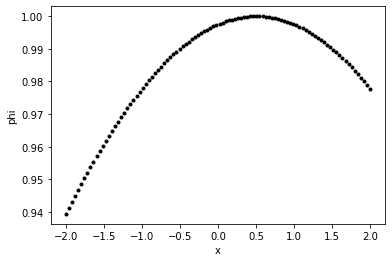
\includegraphics[width=0.3\textwidth]{Post_3_rbfx}}
\subfloat[][Cubic]{
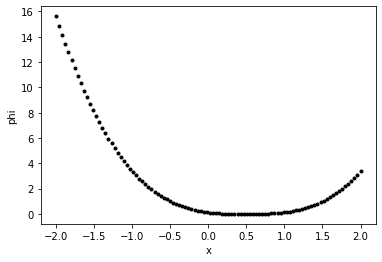
\includegraphics[width=0.3\textwidth]{Post_3_cubicx}}
\subfloat[][Thin Plate Spline]{
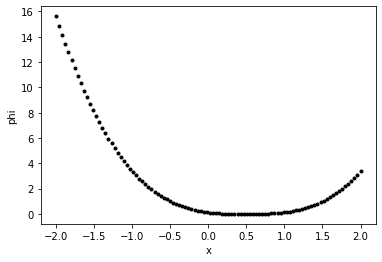
\includegraphics[width=0.3\textwidth]{Post_3_splinex}}
\caption{RBFs in $x$ space with center at $x=0.5$}
\end{figure}

\begin{figure}
\centering
\subfloat[][Gaussian]{
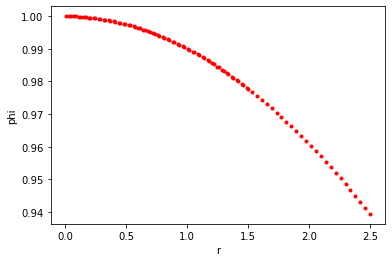
\includegraphics[width=0.3\textwidth]{Post_3_rbfr}}
\subfloat[][Cubic]{
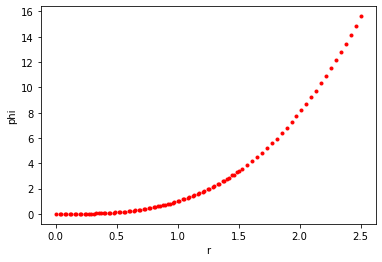
\includegraphics[width=0.3\textwidth]{Post_3_cubicr}}
\subfloat[][Thin Plate Spline]{
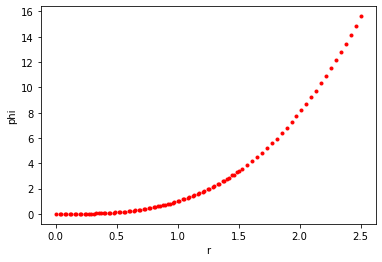
\includegraphics[width=0.3\textwidth]{Post_3_spliner}}
\caption{RBFs in $r$ space}
\end{figure}

\section{Toy Problem}

Now that we have seen the RBF work on a single point, let's take a toy example problem $f(x)=x^2+x+1+U(0,y/2)$ and model it using the gaussian RBF. This can of course be generalized to multi-dimensional problems by making $r$ reflect a multi-dimensional distance metric, but for simplicity (and Christmas Spirit$^{TM}$) we will be in a single dimension. 

\vspace{5mm}

Using Equation (1) as a guide, we know that to solve linear regression problems that "look" like an RBF activation chain we solve $w=(\bm{X}^T \bm{X})^{-1}\bm{X}^T Y$. Therefore, defining $\bm{\Phi}(X) = \phi(x,x')$ for all $x,x'=1...N$ training data, we can solve for the coefficients in Equation (1). In the same way we solved for the maximum likelihood of a multi-dimensional linear regression problem, we solve for the maximum likelihood of a multi-point transformed regression problem. 

\begin{equation}
 \lambda=(\bm{\Phi}^T \bm{\Phi})^{-1}\bm{\Phi}^T Y
\end{equation}

\vspace{5mm}

You will sometimes see Equation (1) written in matrix form with $\bm{\Phi} = \phi(x_i,X_j)$ for testing data $x_i$ and training data $X_j$. I will drop the bolding now, I just wanted to make it clear we are talking about matrices. Below I have provides some examples of 3 training data points on the toy problem where the solution $\lambda$ has been solved for and predictions $\hat{y}$ are in red.

\begin{align*}
\hat{y}=\Phi \lambda
\end{align*}

\begin{figure}[h]
\centering
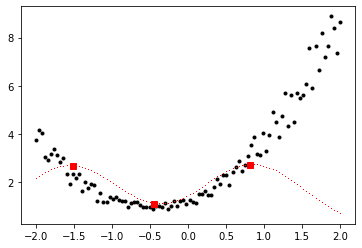
\includegraphics[width=0.3\textwidth]{Post_3_rand1}
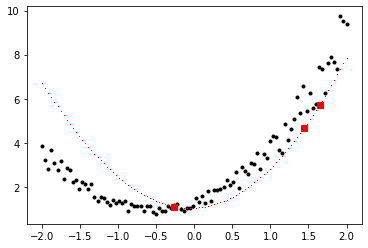
\includegraphics[width=0.3\textwidth]{Post_3_rand2}
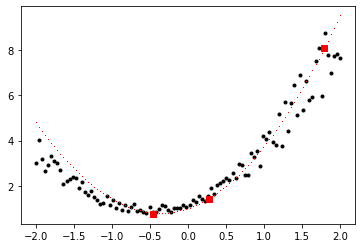
\includegraphics[width=0.3\textwidth]{Post_3_rand3}
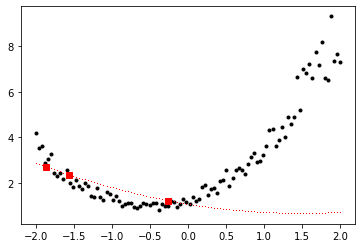
\includegraphics[width=0.3\textwidth]{Post_3_rand4}
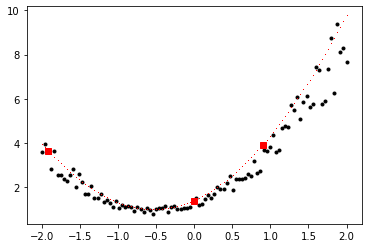
\includegraphics[width=0.3\textwidth]{Post_3_rand5}
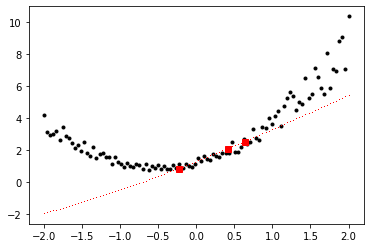
\includegraphics[width=0.3\textwidth]{Post_3_rand6}
\caption{Regression w/ Random Training Data}
\end{figure}

\section{Classification}

If we would like to solve a classification problem, say $y \in \{1,-1\}$, we modify Equation (1):

\begin{equation}
\hat{y}=sign\{\Sigma_{i=1}^{n_c} \lambda_i \phi(r_i)\}
\end{equation}

\begin{equation}
y(x) = 1 \ast \{x^2+x+1 \ge 2 \}
\end{equation}

In this example, the actual function $f(x)$ is hidden and we only have access to the class $y \in \{1,-1\}$. Here we train $\lambda$ and predict $\hat{y}$ the same as in regression problems. In Figure 4 a regression problem is posed as the classification problem.

\vspace{15mm}

\begin{figure}[h]
\centering
\subfloat[][Regression]{
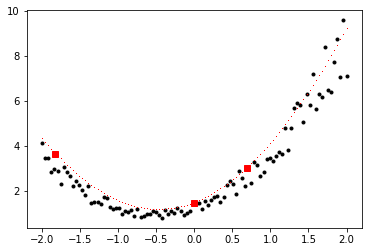
\includegraphics[width=0.3\textwidth]{Post_3_class1}}
\subfloat[][Classification]{
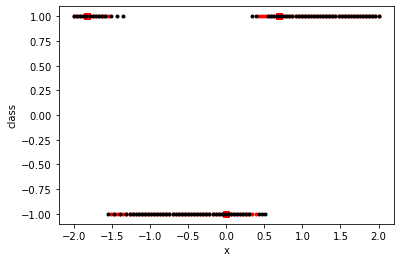
\includegraphics[width=0.3\textwidth]{Post_3_class2}}
\caption{Classification w / Random Training Data | red squares = training data, red dots = predictions}
\end{figure}

\section{Polynomial Terms}

A common practice to improve prediction with RBFs is to add a polynomial term:

\begin{equation}
\hat{y}=\Sigma_{i=1}^{n_c} \lambda_i \phi(r_i)+ p(x)
\end{equation}

So for example we would have $\hat{y}=\Sigma_{i=1}^{n_c} \lambda_i \phi(r_i)+c_0+c_1(x)$ for a linear term and bias for a single variable. To solve for this we solve $A\Lambda=\gamma$ with $P$ being rows of training data $[1\:X_1 ... X_N]$ and $\gamma=[y\:0]$. The regression results are shown.

\begin{align*}
A = 
\begin{pmatrix}
\Phi & P \\
P^T & 0 \\
\end{pmatrix}
\end{align*}

\begin{align*}
\Lambda = 
\begin{pmatrix}
\lambda \\
c \\
\end{pmatrix}
\end{align*}

\begin{figure}[h]
\centering
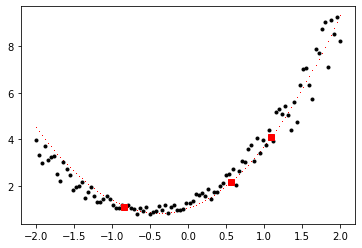
\includegraphics[width=0.3\textwidth]{Post_3_linearterm}
\caption{Regression w / RBF + $c_0+c_1x$ Term}
\end{figure}

\section{Hyperparameters for RBFs}

We will then chose the best hyperparameters $\sigma$ by varying $\sigma$ and picking the parameter with the lowest out-of-sample error. Here I will skip any cross-validation procedure and show the correct randomized error for various values. 

\begin{figure}[h]
\centering
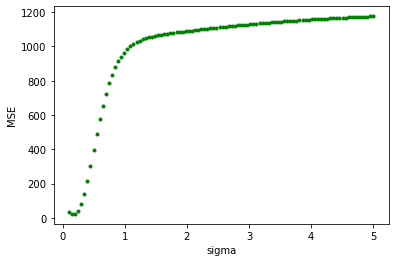
\includegraphics[width=0.6\textwidth]{Post_3_sigma}
\caption{Mean Squared Error for Various $\sigma$ in RBF Model}
\end{figure}

\vspace{5mm}

We should also look at the number of centers. So far the centers for the RBF have all been the training data, but these can be placed anywhere. Generally, the more centers, the more fit the data is. For example note Figure 7(a). With 2 centers, which is less than the 3 data points, the model becomes a simple linear model. We therefore seek to reduce the number of nodes to the minimum number required. Against one should use cross-validation techniques or other model comparison tools.

\begin{figure}[h]
\centering
\subfloat[][2 Centers]{
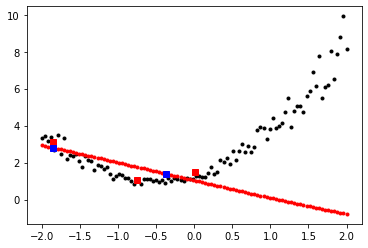
\includegraphics[width=0.3\textwidth]{Post_3_nodes1}}
\subfloat[][3 Centers]{
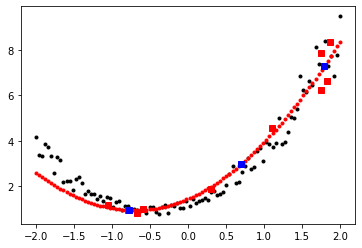
\includegraphics[width=0.3\textwidth]{Post_3_nodes2}}
\caption{RBF Regression for Various Numbers of Centers | data points = red, centers = blue}
\end{figure}

\vspace{5mm}

Okay thank you everyone for reading. Next week we will be talking about MCMC and Bayesian Methods a bit. Have a safe and fun holiday!

\end{document}